\documentclass[main.tex]{subfiles}

\begin{document}

\section{Aufgabe 2}
Bei einer Population von $30$ Versuchstieren wird an einem bestimmten Tag das Gewicht (in kg) gemessen. Dabei ergaben sich die folgenden Messungen:
\begin{center}
\begin{tabular}{cccccccccc}
$12,16$ & $11,53$ & $14,02$ & $11,85$ & $10,94$ & $11,83$ & $12,94$ & $11,46$ & $13,15$ & $12,70$ \\
$10,88$ & $13,24$ & $14,04$ & $10,95$ & $14,78$ & $12,39$ & $13,69$ & $11,82$ & $14,28$ & $12,96$ \\
$13,24$ & $13,42$ & $12,23$ & $15,04$ & $11,34$ & $12,28$ & $13,42$ & $13,93$ & $14,73$ & $11,28$
\end{tabular}
\end{center}
\begin{enumerate}
\item Erstellen Sie zur Übersicht der Verteilung eine Tabelle mit der Klasseneinteilung $[10,0;11,5)$, $[11,5;13,0)$, $[13,0;14,0)$, $[14,0;16,0)$. Geben Sie die absolute und relative Klassenhäufigkeit sowie die Werte für die empirische Verteilungsfunktion an.
\item Zeichnen Sie
\begin{enumerate}
\item das zugehörige Histogramm und
\item die empirische Verteilungsfunktion.
\end{enumerate}
\item Berechnen Sie aus den klassierten Daten
\begin{enumerate}
\item das arithmetische Mittel
\item den Median
\item die Modalklasse
\item das 90\% -Quantil
\item das untere Quartil
\item die empirische Varianz sowie die empirische Standardabweichung
\end{enumerate}
\item Geben Sie den Variationskoeffizienten an.
\end{enumerate}

\subsection{Lösung 2}

\begin{center}
\begin{tabular}{l|c|c|c|c}
Klasse & Absolute Häufigkeit & relative H.   & emp. Verteilungsf.       & Dichte\\
$A_j$  & $n_j$               & $h_j$         & $H_j$                    & $\frac{n_j}{\abs{A_j}}$ \\\hline
$[10,0;\  11,5)$  & 6                   & 0,200               & 0,200   &  $4$              \\
$[11,5;\  13,0)$  & 11                  & 0,367               & 0,567   &  $7,\overline{3}$ \\
$[13,0;\  14,0)$  & 7                   & 0,233               & 0,800   &  $7$              \\
$[14,0;\  16,0)$  & 6                   & 0,200               & 1,000   &  $3$              \\
\end{tabular}
\end{center}

\begin{figure}[h!]
    \begin{center}
        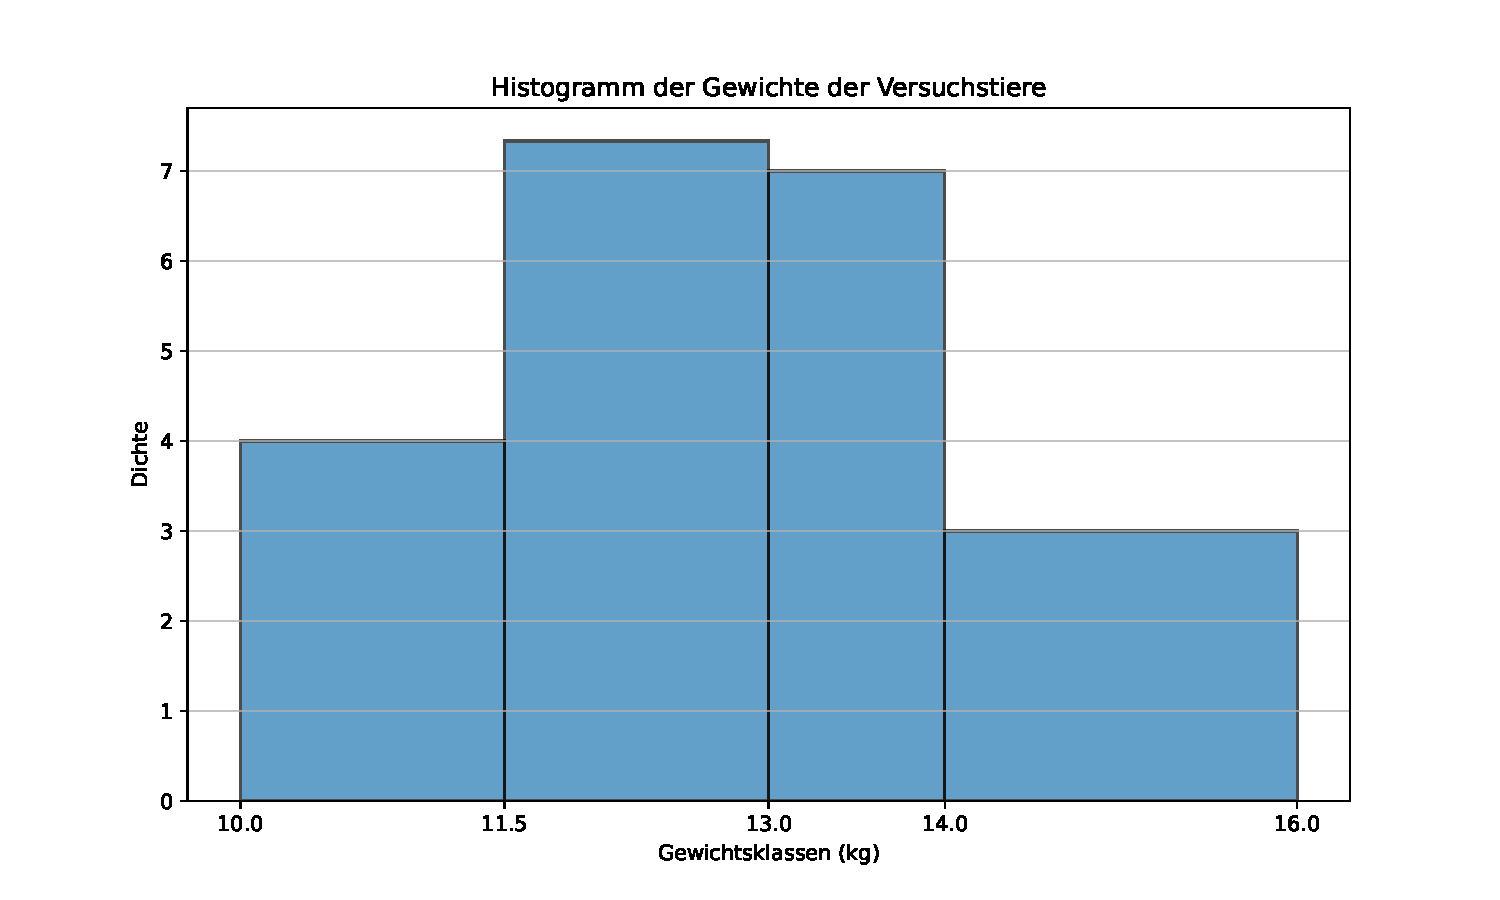
\includegraphics[width=1\textwidth]{A2-b.pdf}
        \caption{Lösung der Aufgabe 2b) i.}
    \end{center}
\end{figure}

\begin{figure}[h!]
    \begin{center}
        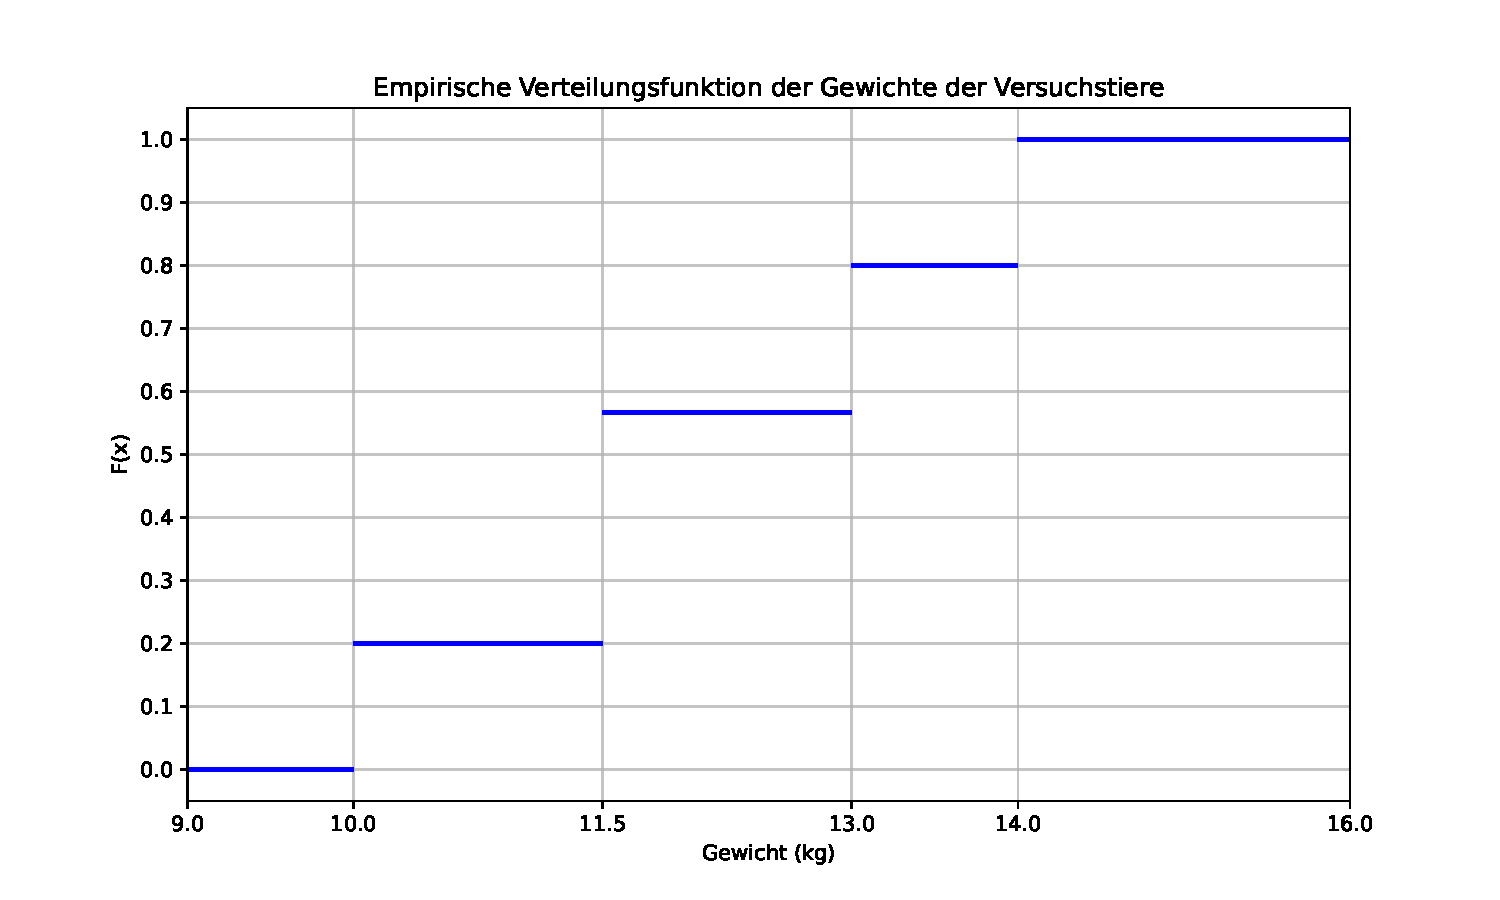
\includegraphics[width=1\textwidth]{A2-b2.pdf}
        \caption{Lösung der Aufgabe 2b) ii.}
    \end{center}
\end{figure}

\renewcommand{\labelenumi}{\theenumi}
\renewcommand{\theenumi}{\roman{enumi}.}%
\begin{enumerate}
    \item Das arithmetische Mittel der Gewichte beträgt $\overline{x}=\frac{77}{25} = 12,79$ kg.
    \item Der empirische Median der Gewichte ist $\tilde{x}\approx 12,72$ kg.
    \item Die Modalklasse ist die Klasse mit der größten Häufigkeitsdichte, also die Klasse mit der höchsten Anzahl an Datenpunkten im Verhältnis zur Klassengröße. Hier ist das $A_2 = [11,5;\  13,0)$.
    \item Das $90\%$-Quantil der Gewichte liegt bei $x_{0,9} = 15$ kg. Das bedeutet, dass 90\% der Gewichte unter diesem Wert liegen.
    \item Das untere Quartil liegt bei $x_{0,25} \approx 11,7$ kg. Das bedeutet, dass 25\% der Gewichte unter oder gleich diesem Wert sind.
    \item Die empirische Varianz beträgt $s^2 = 2,1$ kg$^2$ und die empirische Standardabweichung $s \approx 1,45$.
\end{enumerate}

Der Variationskoeffizienten $V$, drückt das Verhältnis der Standardabweichung zum Mittelwert aus und ist ein Maß für die relative Streuung der Daten.
$$
    V = \frac{s}{\overline{x}} = 0,1134
$$

\end{document}
